\documentclass[../main-physics-problems.tex]{subfiles}
\begin{document}

\subsection{Changing Momentum}
\subsubsection{Relating Change in Momentum to Change in Velocity}
\subsubsection{The Relationship between Net Force and Momentum}
\subsubsection{The Relationship between Time and Momentum}
\subsubsection{Real-Life Applications of Impulse and Momentum}
\subsubsection{Solving Problems Using the Impulse-Momentum Theorem}
\subsection{Changing Kinetic Energy}
\subsubsection{Identifying if a Net Force is Doing Work}
\subsubsection{Calculating Net Work}
\subsubsection{The Relationship between Net Force and Kinetic Energy}
\subsubsection{The Relationship between Displacement and Kinetic Energy}
\subsubsection{Solving Problems using the Work-Energy Theorem}
\subsubsection{Comparing the Power of Various Situations}
\subsubsection{Calculating Power}

\begin{questions}
\question
A force causes a \SI{70}{kg} football player to change his velocity by \SI{10}{m/s}. Determine the change in momentum experienced by the player.

\begin{randomizechoices}
    \correctchoice \SI{70}{kg\cdot m/s}
    \choice \SI{7}{kg\cdot m/s}
    \choice \SI{0.7}{kg\cdot m/s}
\end{randomizechoices}

\question
A player twice the mass of the first (\SI{140}{kg}) experiences the same change in momentum.  Would his change in change in velocity be higher, lower or the same as the first player?  Explain.

\begin{randomizechoices}
    \correctchoice lower
    \choice higher
    \choice the same
\end{randomizechoices}

\question
A car with a mass of \SI{1000}{kg} is at rest at a stop light.  When the light turns green, it is pushed by a net force of \SI{2000}{N} for \SI{10}{s}. What is the car's change in velocity?

\begin{randomizechoices}
    \correctchoice \SI{20}{m/s}
    \choice \SI{0.05}{m/s}
    \choice \SI{2}{m/s}
\end{randomizechoices}

\begin{solution}
\begin{equation*}
    F_\mathrm{net} \Delta t = \Delta p = m \Delta v
\end{equation*}

\begin{equation*}
    \Delta v = \frac{F_\mathrm{net}\Delta t}{m} = \boxed{\SI{20}{m/s}}
\end{equation*}
\end{solution}

\question
A car with a mass of \SI{1000}{kg} is at rest at a stop light. When the light turns green, it is pushed by a net force of \SI{2000}{N} for \SI{10}{s}. What is the car's change in momentum?

\begin{randomizechoices}
    \correctchoice \SI{20000}{kg\cdot m/s}
    \choice \SI{200}{kg\cdot m/s}
    \choice \SI{2000}{kg\cdot m/s}
\end{randomizechoices}

\begin{solution}
\begin{equation*}
    \Delta p = F_\mathrm{net} \Delta t = \boxed{\SI{20000}{kg\cdot m/s}}
\end{equation*}
\end{solution}

\question
A car with half the mass of the previous car (\SI{500}{kg}) is at rest at a stop light.  When the light turns green, it is pushed by the same net force for the same amount of time (\SI{2000}{N} for \SI{10}{s}). How will the less massive car's change in velocity compare with that of the first car? 

\begin{randomizechoices}
    \correctchoice It will be larger.
    \choice It will be smaller. 
    \choice It will be the same.
\end{randomizechoices}

\question
A car with half the mass of the previous car (\SI{500}{kg}) is at rest at a stop light.  When the light turns green, it is pushed by the same net force for the same amount of time (\SI{2000}{N} for \SI{10}{s}). How will the less massive car's change in momentum compare with that of the first car? 

\begin{randomizechoices}
    \correctchoice It will be the same. 
    \choice It will be larger.
    \choice It will be smaller.
\end{randomizechoices}

\question
An object is moving with a velocity of \SI{4}{m/s}, and it speeds up to a velocity of \SI{19}{m/s} in \SI{5}{s}. If its mass is \SI{7}{kg}, what net force acted upon it?

\begin{randomizechoices}
    \correctchoice \SI{21}{N}
    \choice \SI{15}{N}
    \choice \SI{28}{N}
    \choice \SI{105}{N}
\end{randomizechoices}

\question
A car with a mass of \SI{1000}{kg} has a velocity of \SI{38}{m/s}. The brakes are applied, and the car stops in 4 seconds. Determine the net force applied to the car during that time.

\begin{randomizechoices}
    \correctchoice \SI{-9500}{N}
    \choice \SI{-9.5}{N}
    \choice \SI{9.5}{N}
    \choice \SI{9500}{N}
\end{randomizechoices}


\question
A car with a mass of \SI{1000}{kg} has a velocity of \SI{38}{m/s}. The brakes are applied, and the car stops in 4 seconds. What is the change in momentum?

\begin{randomizechoices}
    \correctchoice \SI[group-separator={,}]{-38000}{kg\cdot m/s}
    \choice \SI[group-separator={,}]{38000}{kg\cdot m/s}
    \choice \SI{-9500}{kg\cdot m/s}
    \choice \SI{9500}{kg\cdot m/s}
\end{randomizechoices}

\question
The same car as before (with a mass of \SI{1000}{kg} and a velocity of \SI{38}{m/s}) takes twice the amount of time to stop (8 seconds). How does the applied force compare to the first time? 

\begin{randomizechoices}
    \correctchoice It is lesser.
    \choice It is greater.
    \choice It is the same.
\end{randomizechoices}

\question
The same car as before (with a mass of \SI{1000}{kg} and a velocity of \SI{38}{m/s}) takes twice the amount of time to stop (8 seconds). How does the car’s change in momentum compare to the first time? 

\begin{randomizechoices}
    \correctchoice It is the same.
    \choice It is higher.
    \choice It is lower.
\end{randomizechoices}

\question
Momentum is \fillin[a vector][4cm]\ quantity.

\begin{randomizechoices}[norandomize]
    \correctchoice a vector
    \choice a scalar
    \choice both a vector and scalar
    \choice neither vector nor scalar
\end{randomizechoices}

\question
Consider the mass and velocity values of Objects A and B below.

\begin{center}
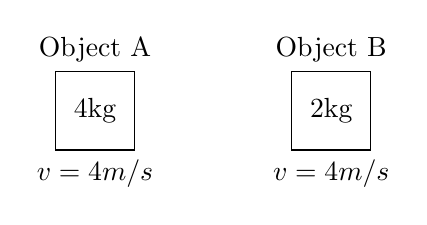
\begin{tikzpicture}
    \draw (0,0) rectangle (1,1) node[pos=0.5,above=5mm] {Object A} node[pos=0.5] {\SI{4}{kg}} node[pos=0.5,below=5mm] {$v = \SI{4}{m/s}$};
    \draw[xshift=3cm] (0,0) rectangle (1,1) node[pos=0.5,above=5mm] {Object B} node[pos=0.5] {\SI{2}{kg}} node[pos=0.5,below=5mm] {$v = \SI{4}{m/s}$};
\end{tikzpicture}
\end{center}

The momentum of Object A is $p_A$, and the momentum of object B is $p_B$. What is the ratio the momentum of Object A to that of Object B, $p_A : p_B$?

\begin{randomizechoices}
    \correctchoice $2:1$
    \choice $1:2$
    \choice $1:1$
    \choice $4:1$
\end{randomizechoices}
\end{questions}


\textbf{Work}
\begin{questions}

\question
The diagram below shows the net force applied to a box vs the box's displacement. How much work was done on the box over its \SI{20}{m} displacement?

\begin{center}
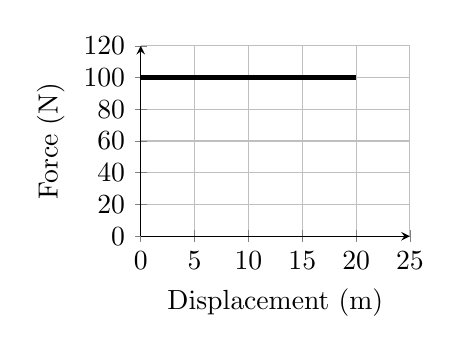
\begin{tikzpicture}
    \begin{axis}[height=4cm,width=5cm,
        axis lines=left,
        ylabel={Force (N)},
        xlabel={Displacement (m)},
        ymin=0,ymax=120,
        xmin=0,xmax=25,
        ytick={0,20,...,120},
        xtick={0,5,...,25},
        grid
        ]
        \addplot[ultra thick] coordinates{(0,100)(20,100)};
    \end{axis}
\end{tikzpicture}
\end{center}

\begin{randomizechoices}
    \correctchoice \SI{2000}{J}
    \choice \SI{200}{J}
    \choice \SI{5000}{J}
    \choice \SI{500}{J}
\end{randomizechoices}

\question
A \SI{200}{kg} crate is lifted to a \SI{3}{m} high platform by a forklift. Assuming that it was lifted with a net force of \S{10}{N}, how much net work was done on the crate?

\begin{randomizechoices}
    \correctchoice \SI{30}{J}
    \choice \SI{2000}{J}
    \choice \SI{600}{J}
    \choice \SI{60}{J}
\end{randomizechoices}

\question
A person exerted a force of \SI{9000}{N} on a stalled car for 30 seconds but was unable to move it. What is the net force acting on the car?

\begin{randomizechoices}[keeplast]
    \correctchoice \SI{0}{N}
    \choice \SI{9000}{N}
    \choice Net force cannot be determined without knowing the frictional force on the car.
\end{randomizechoices}

\question
A person exerted a force of \SI{9000}{N} on a stalled car for 30 seconds but was unable to move it. What is the net work acting on the car?

\begin{randomizechoices}[keeplast]
    \correctchoice \SI{0}{J}
    \choice \SI{9000}{J}
    \choice Net work cannot be determined without knowing the frictional force on the car.
\end{randomizechoices}

\question
A person lifts a \SI{0.5}{kg} flowerpot with a force of \SI{7}{N}, while the Earth pulls down on it (gravitational force) with \SI{5}{N}. The person places it on a \SI{1}{m} high shelf. How much net work was done getting the flowerpot onto the shelf?

\begin{randomizechoices}
    \correctchoice \SI{2}{J}
    \choice \SI{5}{J}
    \choice \SI{7}{J}
    \choice \SI{0}{J}
\end{randomizechoices}

\question
In Case 1 below, a force is exerted at \ang{30} above the horizontal as a box is displaced by some amount. In Case 1, the same force is applied across the same displacement, but the angle is \ang{60} above the horizontal. The work done in the first case is $W_1$, and the work done in the second case is $W_2$. What is the ratio $\frac{W_1}{W_2}$?

\begin{center}
\begin{tikzpicture}[x=1.4cm,y=1.4cm]
    \draw (0,0) -- (5.5,0);
    \draw (2,0) rectangle ++(1.5,1);
    \draw[dashed] (3.5,0.5) -- ++(1.5,0);
    \draw[thick,->] (3.5,0.5) -- ++({1.5*cos(30)},{1.5*sin(30)}) node[above,pos=0.7] {$F$};
    \node[above] at (4.2,0.5) {\ang{30}};
\end{tikzpicture}

\vspace{1em}

\begin{tikzpicture}[x=1.4cm,y=1.4cm]
    \draw (0,0) -- (5.5,0);
    \draw (2,0) rectangle ++(1.5,1);
    \draw[dashed] (3.5,0.5) -- ++(1.5,0);
    \draw[thick,->] (3.5,0.5) -- ++({1.5*cos(60)},{1.5*sin(60)}) node[left,pos=0.9] {$F$};
    \node[above] at (3.9,0.5) {\ang{60}};
\end{tikzpicture}
\end{center}

\clearpage

\question
In the following procedure, you will record time, position, and velocity data of a falling object so that you can then measure energy and work on the ball. 

\begin{itemize}[itemsep=0pt,topsep=0pt]
    \item basketball and volleyball
    \item digital scale
    \item motion detector
    \item ruler
\end{itemize}
% \end{multicols}

\bigskip

\begin{parts}
\part Measure the masses of Ball 1 and Ball 2:

\smallskip

\begin{center}
    Ball 1 mass: \rule{2cm}{0.15mm}\,kg \hspace{4em}
    Ball 2 mass: \rule{2cm}{0.15mm}\,kg
\end{center}
\part Go to \texttt{graphicalanalysis.app}, click \texttt{Sensor Data Collection}, and connect the motion detector using the \texttt{Wireless} option.
\part Press \texttt{Collect}. Then drop a ball from rest from about 1.5 meters above the detector and get a partner to catch the ball about 0.5 meters above the detector.
\part Record time, position, and velocity data in the following table for the first ball:

\bgroup
\def\arraystretch{1.5}%
\textbf{Ball 1 Data}:
\begin{center}
\begin{tabular}{|c|c|c|c|c|}
    \hline
    \textbf{Location} & \textbf{Time} (s) & \textbf{Position} (m) & \textbf{Velocity} (m/s) & \textbf{Kinetic Energy} (J) \\ \hline
    At release & \hspace{2.5cm} & \hspace{2.5cm} & \hspace{2.5cm} & \\ \hline
    Before catch & & & & \\ \hline
\end{tabular}
\end{center}
\egroup

\part Repeat the same measurements for the second ball:

\bgroup
\def\arraystretch{1.5}%
\textbf{Ball 2 Data}:
\begin{center}
\begin{tabular}{|c|c|c|c|c|}
    \hline
    \textbf{Location} & \textbf{Time} (s) & \textbf{Position} (m) & \textbf{Velocity} (m/s) & \textbf{Kinetic Energy} (J) \\ \hline
    At release & \hspace{2.5cm} & \hspace{2.5cm} & \hspace{2.5cm} & \\ \hline
    Before catch & & & & \\ \hline
\end{tabular}
\end{center}
\egroup

\part Use the kinetic energies to calculate the change in kinetic energy of each ball:

\bgroup
\def\arraystretch{3}%
\begin{center}
\begin{tabular}{|c|c|}
    \hline
    \textbf{Object} & \textbf{Change in kinetic energy} (J) \\ \hline
    Ball 1 & \hspace{12cm} \\ \hline
    Ball 2 & \\ \hline
\end{tabular}
\end{center}
\egroup

\part The force of gravity on an object, in newtons, is approximately equal to the object's mass in kilograms multiplied by 10. Calculate the gravitatioanl force on each ball.

\bgroup
\def\arraystretch{3}%
\begin{center}
\begin{tabular}{|c|c|}
    \hline
    \textbf{Object} & \textbf{Force of gravity} (N) \\ \hline
    Ball 1 & \hspace{12cm} \\ \hline
    Ball 2 & \\ \hline
\end{tabular}
\end{center}
\egroup

\clearpage
\part 
Use the net force and position data to find the work done on the ball by gravity:

\bgroup
\def\arraystretch{3}%
\begin{center}
\begin{tabular}{|c|c|c|}
    \hline
    \textbf{Object} & \textbf{Distance traveled} (m) & \textbf{Work} (J) \\ \hline
    Ball 1 &\hspace{5cm} & \hspace{8cm} \\ \hline
    Ball 2 & &\\ \hline
\end{tabular}
\end{center}
\egroup

\end{parts}
    
\end{questions}

\clearpage

\begin{questions}
\question
The object's mass is \SI{12}{kg}. Calculate the change in velocity, change in momentum, and change in kinetic energy. 

\begin{center}
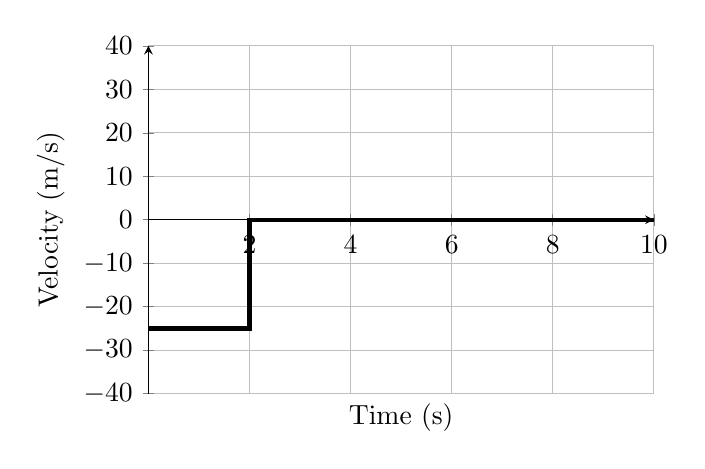
\begin{tikzpicture}
    \begin{axis}[height=6cm,width=8cm,
        axis y line=left,
        axis x line=center,
        ylabel={Velocity (m/s)},
        xlabel={Time (s)},
        x label style={at={(axis description cs:0.5,0)},anchor=north},
        ymin=-40,ymax=40,
        xmin=0,xmax=10,
        ytick={-40,-30,...,40},
        xtick={0,2,...,10},
        grid=both,
        clip=false
    ]
        \addplot[ultra thick] coordinates {(0,-25)(2,-25)(2,0)(10,0)};
    \end{axis}
\end{tikzpicture}
\end{center}

\begin{solution}
\begin{align*}
    \Delta v &= v_f - v_i \\[1ex]
    &= \SI{0}{m/s} - (\SI{-25}{m/s}) \\[1ex]
    &= \boxed{\SI{25}{m/s}} \\[2ex]
    %
    \Delta p &= m \Delta v \\[1ex]
    &= (\SI{12}{kg})(\SI{25}{m/s}) \\[1ex]
    &= \boxed{\SI{300}{kg\cdot m/s}} \\[2ex]
    %
    \Delta \mathrm{KE} &= \mathrm{KE}_f - \mathrm{KE}_i \\[1ex]
    &= \frac{1}{2}m v_f^2 - \frac{1}{2}mv_i^2 \\[1ex]
    &= \frac{1}{2}(\SI{12}{kg})(\SI{0}{m/s})^2 - \frac{1}{2}(\SI{12}{kg}) (\SI{-25}{m/s})^2 \\[1ex]
    &= \boxed{\SI{-3750}{J}}
\end{align*}


\end{solution}


\ifprintanswers
    \clearpage
\fi

\question
The mass is \SI{20}{kg}. Calculate the change in velocity, change in momentum, and change in kinetic energy. 

\begin{center}
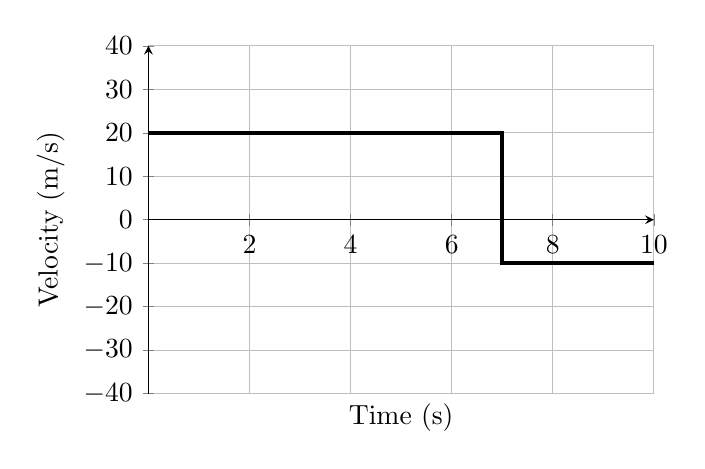
\begin{tikzpicture}
    \begin{axis}[height=6cm,width=8cm,
        axis y line=left,
        axis x line=center,
        ylabel={Velocity (m/s)},
        xlabel={Time (s)},
        x label style={at={(axis description cs:0.5,0)},anchor=north},
        ymin=-40,ymax=40,
        xmin=0,xmax=10,
        ytick={-40,-30,...,40},
        xtick={0,2,...,10},
        grid=both,
        clip=false
    ]
        \addplot[ultra thick] coordinates {(0,20)(7,20)(7,-10)(10,-10)};
    \end{axis}
\end{tikzpicture}
\end{center}

\begin{solution}
\begin{align*}
    \Delta v &= v_f - v_i \\[1ex]
    &= \SI{-10}{m/s} - \SI{20}{m/s} \\[1ex]
    &= \boxed{\SI{-30}{m/s}} \\[2ex]
    %
    \Delta p &= m \Delta v \\[1ex]
    &= (\SI{20}{kg})(\SI{-30}{m/s}) \\[1ex]
    &= \boxed{\SI{-600}{kg\cdot m/s}} \\[2ex]
    %
    \Delta \mathrm{KE} &= \mathrm{KE}_f - \mathrm{KE}_i \\[1ex]
    &= \frac{1}{2}m v_f^2 - \frac{1}{2}mv_i^2 \\[1ex]
    &= \frac{1}{2}(\SI{20}{kg})(\SI{-10}{m/s})^2 - \frac{1}{2}(\SI{20}{kg}) (\SI{20}{m/s})^2 \\[1ex]
    &= \boxed{\SI{-3000}{J}}
\end{align*}
\end{solution}


\ifprintanswers
    \clearpage
\fi
\question
The mass is \SI{40}{kg}. Calculate the change in velocity, change in momentum, and change in kinetic energy. 

\begin{center}
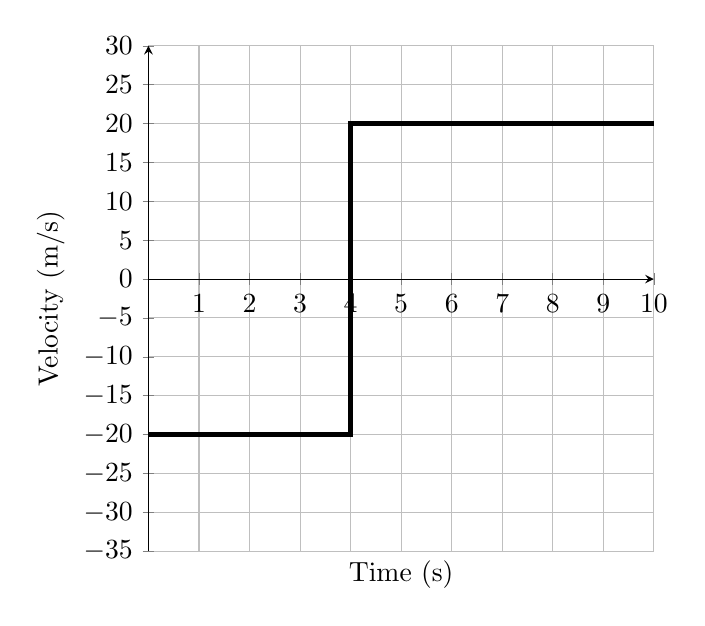
\begin{tikzpicture}
    \begin{axis}[height=8cm,width=8cm,
        axis y line=left,
        axis x line=center,
        ylabel={Velocity (m/s)},
        xlabel={Time (s)},
        x label style={at={(axis description cs:0.5,0)},anchor=north},
        ymin=-35,ymax=30,
        xmin=0,xmax=10,
        ytick={-35,-30,...,30},
        xtick={0,1,...,10},
        grid=both,
        clip=false
    ]
        \addplot[ultra thick] coordinates {(0,-20)(4,-20)(4,20)(10,20)};
    \end{axis}
\end{tikzpicture}
\end{center}

\begin{solution}
\begin{align*}
    \Delta v &= v_f - v_i \\[1ex]
    &= \SI{20}{m/s} - (\SI{-20}{m/s}) \\[1ex]
    &= \boxed{\SI{40}{m/s}} \\[2ex]
    %
    \Delta p &= m \Delta v \\[1ex]
    &= (\SI{40}{kg})(\SI{40}{m/s}) \\[1ex]
    &= \boxed{\SI{1600}{kg\cdot m/s}} \\[2ex]
    %
    \Delta \mathrm{KE} &= \mathrm{KE}_f - \mathrm{KE}_i \\[1ex]
    &= \frac{1}{2}m v_f^2 - \frac{1}{2}mv_i^2 \\[1ex]
    &= \frac{1}{2}(\SI{40}{kg})(\SI{20}{m/s})^2 - \frac{1}{2}(\SI{40}{kg}) (\SI{-20}{m/s})^2 \\[1ex]
    &= \boxed{\SI{0}{J}}
\end{align*}
\end{solution}


\ifprintanswers
    \clearpage
\fi

\question
The mass is \SI{35}{kg}. Calculate the change in velocity, change in momentum, and change in kinetic energy. 

\begin{center}
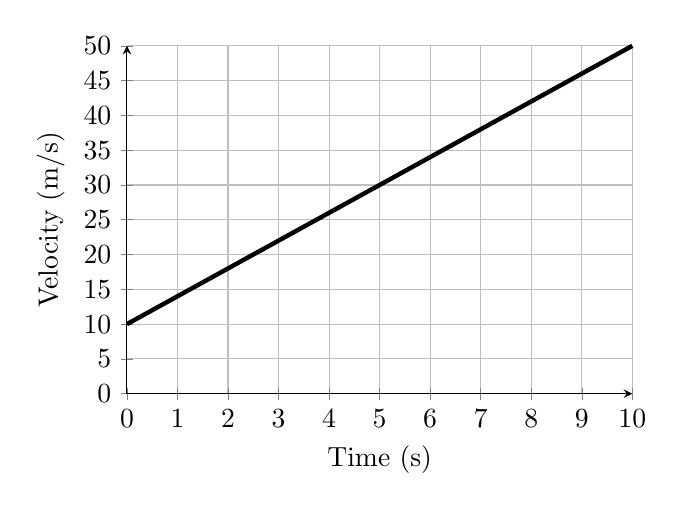
\begin{tikzpicture}
    \begin{axis}[height=6cm,width=8cm,
        axis lines=left,
        ylabel={Velocity (m/s)},
        xlabel={Time (s)},
        ymin=0,ymax=50,
        xmin=0,xmax=10,
        ytick={0,5,...,50},
        xtick={0,1,...,10},
        grid=both,
        clip=false
    ]
        \addplot[ultra thick] coordinates {(0,10)(10,50)};
    \end{axis}
\end{tikzpicture}
\end{center}

\begin{solution}
\begin{align*}
    \Delta v &= v_f - v_i \\[1ex]
    &= \SI{50}{m/s} - \SI{10}{m/s} \\[1ex]
    &= \boxed{\SI{40}{m/s}} \\[2ex]
    %
    \Delta p &= m \Delta v \\[1ex]
    &= (\SI{35}{kg})(\SI{40}{m/s}) \\[1ex]
    &= \boxed{\SI{1400}{kg\cdot m/s}} \\[2ex]
    %
    \Delta \mathrm{KE} &= \mathrm{KE}_f - \mathrm{KE}_i \\[1ex]
    &= \frac{1}{2}m v_f^2 - \frac{1}{2}mv_i^2 \\[1ex]
    &= \frac{1}{2}(\SI{35}{kg})(\SI{50}{m/s})^2 - \frac{1}{2}(\SI{35}{kg}) (\SI{10}{m/s})^2 \\[1ex]
    &= \boxed{\SI{42000}{J}}
\end{align*}
\end{solution}

\ifprintanswers
    \clearpage
\fi

\question
The mass is \SI{5}{kg}. Calculate the change in velocity, change in momentum, and change in kinetic energy. 

\begin{center}
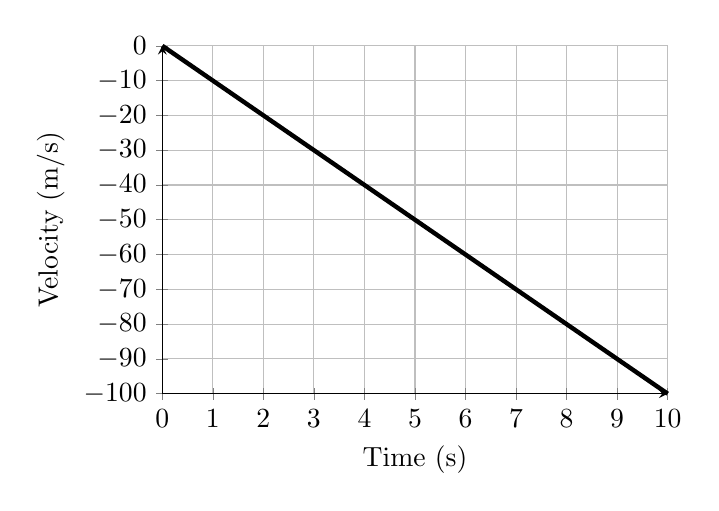
\begin{tikzpicture}
    \begin{axis}[height=6cm,width=8cm,
        axis lines=left,
        ylabel={Velocity (m/s)},
        xlabel={Time (s)},
        %x label style={at={(axis description cs:0.5,0)},anchor=north},
        ymin=-100,ymax=0,
        xmin=0,xmax=10,
        ytick={-100,-90,...,0},
        xtick={0,1,...,10},
        grid=both,
        clip=false
    ]
        \addplot[ultra thick] coordinates {(0,0)(10,-100)};
    \end{axis}
\end{tikzpicture}
\end{center}

\begin{solution}
\begin{align*}
    \Delta v &= v_f - v_i \\[1ex]
    &= \SI{0}{m/s} - \SI{100}{m/s} \\[1ex]
    &= \boxed{\SI{-100}{m/s}} \\[2ex]
    %
    \Delta p &= m \Delta v \\[1ex]
    &= (\SI{5}{kg})(\SI{-100}{m/s}) \\[1ex]
    &= \boxed{\SI{-500}{kg\cdot m/s}} \\[2ex]
    %
    \Delta \mathrm{KE} &= \mathrm{KE}_f - \mathrm{KE}_i \\[1ex]
    &= \frac{1}{2}m v_f^2 - \frac{1}{2}mv_i^2 \\[1ex]
    &= \frac{1}{2}(\SI{5}{kg})(\SI{-100}{m/s})^2 - \frac{1}{2}(\SI{5}{kg}) (\SI{0}{m/s})^2 \\[1ex]
    &= \boxed{\SI{25000}{J}}
\end{align*}
\end{solution}

\ifprintanswers
    \clearpage
\fi

\question
The mass is \SI{6}{kg}. Calculate the change in velocity, change in momentum, and change in kinetic energy. 

\begin{center}
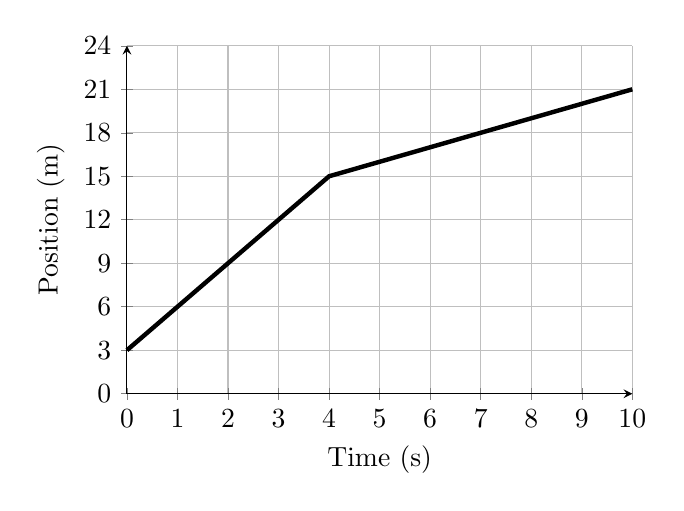
\begin{tikzpicture}
    \begin{axis}[height=6cm,width=8cm,
        axis lines=left,
        ylabel={Position (m)},
        xlabel={Time (s)},
        ymin=0,ymax=24,
        xmin=0,xmax=10,
        ytick={0,3,...,24},
        xtick={0,1,...,10},
        grid=both,
        clip=false
    ]
        \addplot[ultra thick] coordinates {(0,3)(4,15)(10,21)};
    \end{axis}
\end{tikzpicture}
\end{center}

\begin{solution}
\begin{align*}
    \Delta v &= v_f - v_i \\[1ex]
    &= \SI{1}{m/s} - \SI{3}{m/s} \\[1ex]
    &= \boxed{\SI{-2}{m/s}} \\[2ex]
    %
    \Delta p &= m \Delta v \\[1ex]
    &= (\SI{6}{kg})(\SI{-2}{m/s}) \\[1ex]
    &= \boxed{\SI{-12}{kg\cdot m/s}} \\[2ex]
    %
    \Delta \mathrm{KE} &= \mathrm{KE}_f - \mathrm{KE}_i \\[1ex]
    &= \frac{1}{2}m v_f^2 - \frac{1}{2}mv_i^2 \\[1ex]
    &= \frac{1}{2}(\SI{6}{kg})(\SI{-1}{m/s})^2 - \frac{1}{2}(\SI{6}{kg}) (\SI{3}{m/s})^2 \\[1ex]
    &= \boxed{\SI{-24}{J}}
\end{align*}
\end{solution}

\ifprintanswers
    \clearpage
\fi

\question
The mass is \SI{12}{kg}. Calculate the change in velocity, change in momentum, and change in kinetic energy. 

\begin{center}
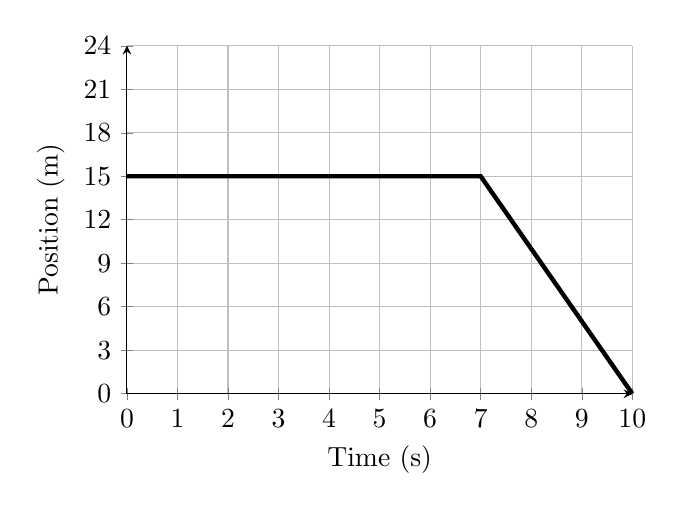
\begin{tikzpicture}
    \begin{axis}[height=6cm,width=8cm,
        axis lines=left,
        ylabel={Position (m)},
        xlabel={Time (s)},
        ymin=0,ymax=24,
        xmin=0,xmax=10,
        ytick={0,3,...,24},
        xtick={0,1,...,10},
        grid=both,
        clip=false
    ]
        \addplot[ultra thick] coordinates {(0,15)(7,15)(10,0)};
    \end{axis}
\end{tikzpicture}
\end{center}


\begin{solution}
\begin{align*}
    \Delta v &= v_f - v_i \\[1ex]
    &= \SI{-5}{m/s} - \SI{0}{m/s} \\[1ex]
    &= \boxed{\SI{-5}{m/s}} \\[2ex]
    %
    \Delta p &= m \Delta v \\[1ex]
    &= (\SI{12}{kg})(\SI{-5}{m/s}) \\[1ex]
    &= \boxed{\SI{-60}{kg\cdot m/s}} \\[2ex]
    %
    \Delta \mathrm{KE} &= \mathrm{KE}_f - \mathrm{KE}_i \\[1ex]
    &= \frac{1}{2}m v_f^2 - \frac{1}{2}mv_i^2 \\[1ex]
    &= \frac{1}{2}(\SI{12}{kg})(\SI{-5}{m/s})^2 - \frac{1}{2}(\SI{12}{kg}) (\SI{0}{m/s})^2 \\[1ex]
    &= \boxed{\SI{150}{J}}
\end{align*}
\end{solution}

\ifprintanswers
    \clearpage
\fi

\question
The object's mass is \SI{14}{kg}. Calculate the change in velocity, change in momentum, and change in kinetic energy.

\begin{center}
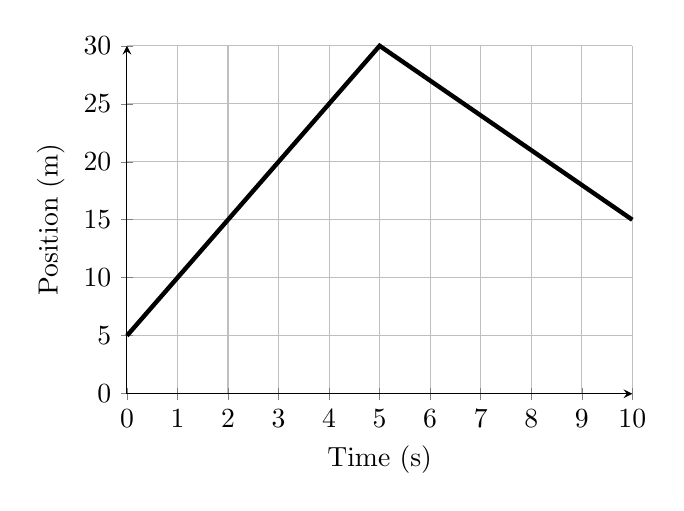
\begin{tikzpicture}
    \begin{axis}[height=6cm,width=8cm,
        axis lines=left,
        ylabel={Position (m)},
        xlabel={Time (s)},
        ymin=0,ymax=30,
        xmin=0,xmax=10,
        ytick={0,5,...,50},
        xtick={0,1,...,10},
        grid=both,
        clip=false
    ]
        \addplot[ultra thick] coordinates {(0,5)(5,30)(10,15)};
    \end{axis}
\end{tikzpicture}
\end{center}

\begin{solution}
\begin{align*}
    \Delta v &= v_f - v_i \\[1ex]
    &= \SI{-3}{m/s} - \SI{5}{m/s} \\[1ex]
    &= \boxed{\SI{-8}{m/s}} \\[2ex]
    \Delta p &= m \Delta v \\[1ex]
    &= (\SI{14}{kg})(\SI{-8}{m/s}) \\[1ex]
    &= \boxed{\SI{-112}{kg\cdot m/s}} \\[2ex]
    \Delta \mathrm{KE} &= \mathrm{KE}_f - \mathrm{KE}_i \\[1ex]
    &= \frac{1}{2}m v_f^2 - \frac{1}{2}mv_i^2 \\[1ex]
    &= \frac{1}{2}(\SI{14}{kg})(\SI{-3}{m/s})^2 - \frac{1}{2}(\SI{14}{kg}) (\SI{5}{m/s})^2 \\[1ex]
    &= \boxed{\SI{-112}{J}}
\end{align*}
\end{solution}

\ifprintanswers
    \clearpage
\fi

\question
A \SI{500}{kg} motorcycle starts from rest and speeds up till it reaches a speed of \SI{30}{m/s}. Calculate the change in velocity, change in momentum, and change in kinetic energy.

\begin{solution}
\begin{align*}
    \Delta v &= v_f - v_i \\[1ex]
    &= \SI{30}{m/s} - \SI{0}{m/s} \\[1ex]
    &= \boxed{\SI{30}{m/s}} \\[2ex]
    %
    \Delta p &= m \Delta v \\[1ex]
    &= (\SI{500}{kg})(\SI{30}{m/s}) \\[1ex]
    &= \boxed{\SI{15000}{kg\cdot m/s}} \\[2ex]
    %
    \Delta \mathrm{KE} &= \mathrm{KE}_f - \mathrm{KE}_i \\[1ex]
    &= \frac{1}{2}m v_f^2 - \frac{1}{2}mv_i^2 \\[1ex]
    &= \frac{1}{2}(\SI{500}{kg})(\SI{30}{m/s})^2 - \frac{1}{2}(\SI{500}{kg}) (\SI{0}{m/s})^2 \\[1ex]
    &= \boxed{\SI{225000}{J}}
\end{align*}
\end{solution}


\ifprintanswers
    \clearpage
\fi

\question 
A \SI{4}{kg} goose is taking off. It starts from rest and then accelerates \SI{3}{m/s^2} for 5 seconds. Calculate the change in velocity, change in momentum, and change in kinetic energy.

\begin{solution}
Since acceleration is defined as

\begin{equation*}
    a = \frac{\Delta v}{\Delta t}
\end{equation*}

it follows that change in velocity is

\vspace{-1em}
\begin{align*}
    \Delta v &= a \Delta t \\[1ex]
    &= (\SI{3}{m/s^2})(\SI{5}{s}) \\[1ex]
    &= \boxed{\SI{15}{m/s}}
\end{align*}
\vspace{-1em}

Therefore,

\begin{align*}
    \Delta p &= m \Delta v \\[1ex]
    &= (\SI{4}{kg})(\SI{15}{m/s}) \\[1ex]
    &= \boxed{\SI{60}{kg\cdot m/s}} \\[2ex]
    %
    \Delta \mathrm{KE} &= \mathrm{KE}_f - \mathrm{KE}_i \\[1ex]
    &= \frac{1}{2}m v_f^2 - \frac{1}{2}mv_i^2 \\[1ex]
    &= \frac{1}{2}(\SI{4}{kg})(\SI{15}{m/s})^2 - \frac{1}{2}(\SI{4}{kg}) (\SI{0}{m/s})^2 \\[1ex]
    &= \boxed{\SI{450}{J}}
\end{align*}
\end{solution}


\ifprintanswers
    \clearpage
\fi

\question
A \SI{0.5}{kg} basketball flies toward the wall at \SI{12}{m/s} in the positive direction. When it hits the wall it bounces backward at \SI{2}{m/s}. Calculate the change in velocity, change in momentum, and change in kinetic energy. 

\begin{solution}
\begin{align*}
    \Delta v &= v_f - v_i \\[1ex]
    &= \SI{-2}{m/s} - \SI{12}{m/s} \\[1ex]
    &= \boxed{\SI{-14}{m/s}} \\[2ex]
    %
    \Delta p &= m \Delta v \\[1ex]
    &= (\SI{0.5}{kg})(\SI{-14}{m/s}) \\[1ex]
    &= \boxed{\SI{-7}{kg\cdot m/s}} \\[2ex]
    %
    \Delta \mathrm{KE} &= \mathrm{KE}_f - \mathrm{KE}_i \\[1ex]
    &= \frac{1}{2}m v_f^2 - \frac{1}{2}mv_i^2 \\[1ex]
    &= \frac{1}{2}(\SI{0.5}{kg})(\SI{-2}{m/s})^2 - \frac{1}{2}(\SI{0.5}{kg}) (\SI{12}{m/s})^2 \\[1ex]
    &= \boxed{\SI{-35}{J}}
\end{align*}
\end{solution}

\ifprintanswers
    \clearpage
\fi

\question
A \SI{500}{kg} motorcycle is driving at \SI{30}{m/s}. The rider sees traffic ahead and slows down. The motorcycle's acceleration is \SI{-2}{m/s^2} for the next 8 seconds. Calculate the change in velocity, change in momentum, and change in kinetic energy. 


\begin{solution}
Since acceleration is defined as

\begin{equation*}
    a = \frac{\Delta v}{\Delta t}
\end{equation*}

it follows that change in velocity is

\vspace{-1em}
\begin{align*}
    \Delta v &= a \Delta t \\[1ex]
    &= (\SI{-2}{m/s^2})(\SI{8}{s}) \\[1ex]
    &= \boxed{\SI{-16}{m/s}}
\end{align*}
\vspace{-1em}

So, the final velocity must be $v_f = v_i + \Delta v = \SI{-14}{m/s}$. Thus,

\begin{align*}
    \Delta p &= m \Delta v \\[1ex]
    &= (\SI{500}{kg})(\SI{-16}{m/s}) \\[1ex]
    &= \boxed{\SI{-8000}{kg\cdot m/s}} \\[2ex]
    %
    \Delta \mathrm{KE} &= \mathrm{KE}_f - \mathrm{KE}_i \\[1ex]
    &= \frac{1}{2}m v_f^2 - \frac{1}{2}mv_i^2 \\[1ex]
    &= \frac{1}{2}(\SI{500}{kg})(\SI{-14}{m/s})^2 - \frac{1}{2}(\SI{500}{kg}) (\SI{30}{m/s})^2 \\[1ex]
    &= \boxed{\SI{-176000}{J}}
\end{align*}
\end{solution}



\end{questions}

\clearpage
\subsection*{Other}

\begin{questions}
\question
What does $\Delta p$ mean?


\question
What is the equation for change in momentum? 


\question \label{Isttuf}
Messi, a soccer player whose mass is \SI{67}{kg}, trots at \SI{3}{m/s}. After attaining the ball, he accelerates to \SI{8}{m/s}. What's Messi's change in momentum? 

\begin{solution}
\SI{335}{kg\,m/s}
\end{solution}


\question \label{1vMk6B}
Initially, a \SI{0.5}{kg} fruit bat travels at \SI{5}{m/s}. If it comes to rest on a tree branch, what is its change in momentum?

\begin{solution}
\SI{-2.5}{kg\,m/s}
\end{solution}

\textbf{Calculate the change in momentum.}

\question \label{VtoBkS}
Mass is \SI{40}{kg}. Final velocity is \SI{1}{m/s}. Initial velocity is \SI{97}{m/s}.

\begin{solution}
\SI{-3840}{kg\,m/s}
\end{solution}

\question \label{fhENr6}
Final velocity is \SI{88}{m/s}. Initial velocity is \SI{22}{m/s}. Mass is \SI{7}{kg}.

\begin{solution}
\SI{462}{kg\,m/s}
\end{solution}


\question \label{MqRZuz}
Initial velocity is \SI{64}{m/s}. Final velocity is \SI{75}{m/s}. Mass is \SI{28}{kg}.

\begin{solution}
\SI{308}{kg\,m/s}
\end{solution}


\question \label{qSPMmV}
Mass is \SI{101}{kg}. Initial velocity is \SI{83}{m/s}. Final velocity is \SI{76}{m/s}. 

\begin{solution}
\SI{-707}{kg\,m/s}
\end{solution}


\question \label{4phY3A}
Initial velocity is \SI{17}{m/s}. Mass is \SI{5}{kg}. Final velocity is \SI{35}{m/s}. 

\begin{solution}
\SI{90}{kg\,m/s}
\end{solution}


\question
What's the equation for net force in terms of momentum and time (the original Newton's 2nd Law)?


\question \label{9CaNPq}
What is the equation for Newton's second law of motion, in terms of mass ($m$), velocity ($v$), and time ($t$)? Assume the mass of the system is constant.

\begin{solution}
$F_{\text{net}} = \frac{m\,\Delta v}{\Delta t}$
\end{solution}

\question
What is impulse?


\question \label{6HJcp6}
Consider two objects of the same mass. If a force of \SI{100}{N}  acts on the first for a duration of \SI{1}{s}  and on the other for a duration of \SI{2}{s}, which object will acquire more momentum?

\begin{solution}
The second object
\end{solution}


\question
When the momentum of an object increases with respect to time, is the net force acting on the object zero or non-zero?


\question \label{ukvCcg}
If both mass and velocity of an object are constant, what can you tell about its impulse?

\begin{solution}
Impulse is zero.
\end{solution}


\question \label{dAVKAB}
How much force would be needed to cause a \SI{17}{kg\,m/s} change in the momentum of an object, if the force acted for 5 seconds?

\begin{solution}
\SI{3.4}{N}
\end{solution}


\question \label{R5mamD}
You hit a tennis ball with a racquet, giving it a velocity of \SI{40}{m/s}. The racquet remained in contact with the ball for \SI{6}{ms}, and the ball has a mass of \SI{0.057}{kg}. What is the magnitude of force that you hit the ball with?

\begin{solution}
\SI{380}{N}
\end{solution}


\question \label{rVq3Tj}
A 2000-kg car is moving at \SI{35}{m/s}. The driver presses the gas pedal for 10 seconds, accelerating the car to a final velocity of \SI{55}{m/}s. What is the magnitude of force that was exerted on the car by the engine?

\begin{solution}
\SI{4000}{N}
\end{solution}


\textbf{Calculate the net force on the object.}

\question \label{4Me32D}
Mass is \SI{0.057}{kg}. Initial velocity is \SI{3}{m/s}. Final velocity is \SI{39}{m/s}. Elapsed time is \SI{8.5e-3}{s}.

\begin{solution}
\SI{241}{N}
\end{solution}

\question \label{LKi6tV}
Initial velocity is \SI{-41}{m/s}. Final velocity is \SI{39}{m/s}. Mass is \SI{0.145}{kg}. Elapsed time is \SI{0.7}{ms}.

\begin{solution}
\SI{16571}{N}
\end{solution}

\question \label{uWU1Cn}
Elapsed time is \SI{6}{s}. Mass is \SI{3}{kg}. Final velocity is \SI{36}{m/s}. Initial velocity is \SI{12}{m/s}.

\begin{solution}
\SI{12}{N}
\end{solution}

\question \label{2doawd}
Final velocity is \SI{5}{m/s}. Mass is \SI{200}{kg}. Initial velocity is \SI{-10}{m/s}.  Elapsed time is \SI{8}{s}.

\begin{solution}
\SI{375}{N}
\end{solution}

\question \label{I7jORB}
Initial velocity is \SI{1}{m/s}. Elapsed time is \SI{2}{s}. Final velocity is \SI{12}{m/s}.  Mass is \SI{10}{kg}.

\begin{solution}
\SI{55}{N}
\end{solution}


\question
When does the net force on an object increase: when $\Delta p$ decreases, when $\Delta t$ increases, or when $\Delta t$ decreases?


\question
Why does it hurt less when you fall on a softer surface?


\question
Cars these days have parts that can crumple or collapse in the event of an accident. How does this help protect the passengers? (\textit{Hint}: Refer to Equation~\ref{e8sC6q}.)


\question \label{e2TgS9}
What is the net force exerted on the tennis ball from Example~\ref{EvkSMv} if the ball and racquet make contact for 7 milliseconds?

\begin{solution}
\SI{489}{N}
\end{solution}

\question \label{2lAWwf}
For how long should a force of \SI{50}{N}  be applied to change the momentum of an object by \SI{12}{kg\,m/s} ?

\begin{solution}
\SI{0.24}{s}
\end{solution}

\question \label{6e43y6}
For how long should a force of \SI{130}{N} be applied to an object of mass \SI{50}{kg} to change its speed from \SI{20}{m/s} to \SI{60}{m/s}?

\begin{solution}
\SI{15.4}{s}
\end{solution}

%%%%%

\question \label{S3zmkv}
In physics, what does work mean?


\question
What is the equation for work?


\question
What is the SI unit for work?


\question
Describe a situation in which a force is exerted for a long time and work is done on an object. Explain.


\question \label{g5xjKT}
Describe a situation in which a force is exerted for a long time but \textit{no work} is done on an object. Explain.


\question \label{Xh4gxC}
Adela does work on a lawn mower when she exerts a constant force of \SI{180}{N} to push the mower \SI{25}{m} horizontally on level ground. What is the work done by Adela?

\begin{solution}
\SI{4500}{J}
\end{solution}

\question \label{ZGiBxy}
A tow truck pushes on a car with a force of \SI{5150}{N}, and the car moves a distance of \SI{8.0}{m}. Calculate the work done on the car.

\begin{solution}
\SI{41200}{J}
\end{solution}

\question \label{MTcEJo}
How much work does a supermarket checkout attendant do on a can of soup he pushes \SI{0.600}{m} horizontally with a force of \SI{5.00}{N}?

\begin{solution}
\SI{3.0}{J}
\end{solution}


\vspace{1em}

\textbf{\ref{T4zIud}--\ref{KU49Fc} Calculate the work when a force causes an object to move some distance.}

\question \label{T4zIud}
Force is \SI{84}{N}. Distance is \SI{32}{m}.

\begin{solution}
\SI{2688}{J}
\end{solution}

\question \label{mroTSQ}
Force is \SI{28}{N}. Distance is \SI{73}{m}.

\begin{solution}
\SI{2044}{J}
\end{solution}


\question \label{1KDZL2}
Force is \SI{91}{N}. Distance is \SI{32}{km}.

\begin{solution}
\SI{2.91e6}{J}
\end{solution}


\question \label{masH3z}
Force is \SI{3}{N}. Distance is \SI{55}{cm}.

\begin{solution}
\SI{1.65}{J}
\end{solution}


\question \label{KU49Fc}
Force is \SI{59}{N}. Distance is \SI{62}{mm}.

\begin{solution}
\SI{3.66}{J}
\end{solution}


\question \label{VMEVDL}
Valent\'{i}n, the 75.0-kg jogger, climbs up some stairs and gains 2.50 meters in height above the ground. What is the work done by Valent\'{i}n in getting up the stairs? 

\begin{solution}
\SI{1838}{J}
\end{solution}


\question \label{OgbvKL}
What amount of work should a weightlifter do to lift a \SI{50.0}{kg} dumbell to a height of \SI{1.25}{m}?

\begin{solution}
\SI{613}{J}
\end{solution}

\question \label{T8C3X0}
The work done to move a box 8.0 meters across a table is 31 joules. What is the net force exerted on the box?

\begin{solution}
\SI{3.88}{N}
\end{solution}

\question \label{7BKGsL}
Dario does \SI{75}{J} of work on a soda can to crush the can by a length of \SI{12}{cm}. What is the net force Dario exerts on the aluminum can?

\begin{solution}
\SI{625}{N}
\end{solution}


\question \label{sRogOc}
The forklift operated by Artemio exerts \SI{6800}{N} of force to do \SI{7500}{J} of work to lift a pallet of coconuts. To what distance above the ground is the pallet lifted? 

\begin{solution}
\SI{1.1}{m}
\end{solution}


%%%%%

\question \label{AlYFHO}
What is the equation for power?


\question
What is SI unit of power?


\question
In the power equation (Eq.~\ref{k6uV1p}), what is the SI unit of time?


\question \label{i4fTLq}
Mabel does \SI{10000}{J} of work on a pulley to lift a TV to the 3rd floor in 2 minutes. Calculate the power generated by Mabel.

\begin{solution}
\SI{83.3}{W}
\end{solution}

\question \label{vJllNv}
Mark also does \SI{10000}{J} of work to lift a TV, but it takes him 5 minutes to lift it to the 3rd floor. What is the power generated by Mark?

\begin{solution}
\SI{33.3}{W}
\end{solution}

\textbf{\ref{G7XVHK}--\ref{bPWZDf} Calculate power.}

\question \label{G7XVHK}
Work is \SI{88}{J}. Time is \SI{48}{s}.

\begin{solution}
\SI{1.83}{W}
\end{solution}

\question \label{CJRoQV}
Work is \SI{810}{J}. Time is \SI{31}{s}.

\begin{solution}
\SI{26.1}{W}
\end{solution}


\question \label{AORjkH}
Work is \SI{72}{J}. Time is \SI{3.1}{ms}.

\begin{solution}
\SI{23225.8}{W}
\end{solution}


\question \label{iKHe2E}
Work is \SI{4.4}{J}. Time is \SI{0.9}{ms}.

\begin{solution}
\SI{4888.9}{W}
\end{solution}


\question \label{bPWZDf}
Work is \SI{7.0}{J}. Time is \SI{55}{ms}.

\begin{solution}
\SI{127.3}{W}
\end{solution}


\question \label{RvNudw}
Ruben's truck delivers \SI{1.49e5}{W} of power while dragging a tree across the road for 15 seconds. What is the work done on the tree?

\begin{solution}
\SI{2.235e6}{J}
\end{solution}

\question \label{b9UIEt}
Hercules generates one millions watts of power while doing \SI{625000}{} joules of work to move a heavy boulder. How how long did Hercules push on the boulder?

\begin{solution}
\SI{0.625}{s}
\end{solution}
\end{questions}

\begin{questions}
\question
A boy pushes his wagon at constant speed along a level sidewalk. The graph below represents the relationship between the horizontal force exerted by the boy and the distance the wagon moves. What is the total work done by the boy in pushing the wagon 4.0 meters?

\begin{center}
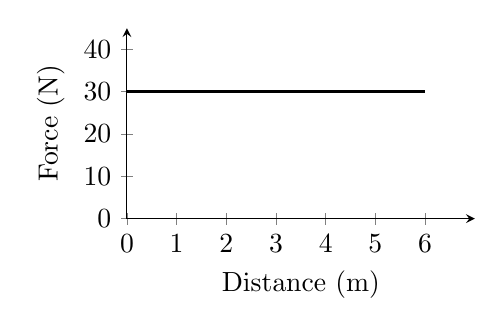
\begin{tikzpicture}
\begin{axis}[width=6cm,height=4cm,
    xmin=0,xmax=7,
    ymin=0,ymax=45,
    clip=false,
    axis lines=left,
    xlabel={Distance (m)},
    ylabel={Force (N)},
    xtick={0,1,...,6},
    ytick={0,10,...,40}
]
\addplot[very thick,
    color=black
    ]
    coordinates{
        (0,30)(6,30)
    };
\end{axis}
\end{tikzpicture}
\end{center}

\begin{randomizechoices}
\choice \SI{7.5}{J}
\correctchoice \SI{120}{J}
\choice \SI{5.0}{J}
\choice \SI{180}{J}
\end{randomizechoices}

\question
A piston, moving through a distance of \SI{0.15}{m}, pushes a box with a mass of \SI{8.0}{kg} onto a conveyor belt with a force of \SI{40}{N}. How much work is done by the piston on the box?

\begin{randomizechoices}
\correctchoice \SI{6.0}{J}
\choice \SI{320}{J}
\choice \SI{5.0}{J}
\choice \SI{120}{J}
\end{randomizechoices}

\question
How many joules of work are done on a box when a force of \SI{25}{N} pushes it \SI{3}{m}?

\begin{randomizechoices}
\choice \SI{3}{J}
\choice \SI{8}{J}
\choice \SI{25}{J}
\correctchoice \SI{75}{J}
\choice \SI{1}{J}
\end{randomizechoices}
\end{questions}
\end{document}

\begin{solution}
\begin{align*}
    \Delta v &= v_f - v_i \\[1ex]
    &= \SI{}{m/s} - \SI{}{m/s} \\[1ex]
    &= \boxed{\SI{}{m/s}} \\[2ex]
    %
    \Delta p &= m \Delta v \\[1ex]
    &= (\SI{}{kg})(\SI{}{m/s}) \\[1ex]
    &= \boxed{\SI{}{kg\cdot m/s}} \\[2ex]
    %
    \Delta \mathrm{KE} &= \mathrm{KE}_f - \mathrm{KE}_i \\[1ex]
    &= \frac{1}{2}m v_f^2 - \frac{1}{2}mv_i^2 \\[1ex]
    &= \frac{1}{2}(\SI{}{kg})(\SI{}{m/s})^2 - \frac{1}{2}(\SI{}{kg}) (\SI{}{m/s})^2 \\[1ex]
    &= \boxed{\SI{}{J}}
\end{align*}
\end{solution}